\section{Cross-chain Atomic Swaps}
\subsection{Terminology}
\begin{itemize}
  \item Cross-Chain Swaps: Trade Ethereum for Bitcoin
  \item Atomic: Ether fully swapped or not at all. 
\end{itemize}
Use case: I want to exchange my 1 BTC to 37 ETH.\\
Obvious approach: use a centralized exchange, such as Binance, Bitstamp, or Kraken.\\
Good Approach: With Atomic Swaps no trust in a centralized platform is needed.

\subsection{Hashed Time-Locked Contracts}
Cryptographic hashing:
\begin{itemize}
  \item one-way function - computationally efficient in one way, computationally highly expensive the other way
  \item deterministic - same input - same output
  \item collision resistant - highly expensive to find two inputs that hash to the same output
\end{itemize}
\subsubsection{Hash lock}
Building block for cross-chain atomic swaps and payment ch
\begin{itemize}
  \item store hashed secret - publicly stored in a smart contract
  \item unlock - only if secret is provided (publicly)
  \item OR: unlock - after timeout
\end{itemize}
Both Chains need to support the same hash function. E.g.: SHA256

\subsubsection{Example}
Now we are ready to do an atomic swap with Alice and Bob with HTLC.
Alice (initiator) creates “secret”, shares with Bob, hash(secret).
Bob now knows hash(secret).\\
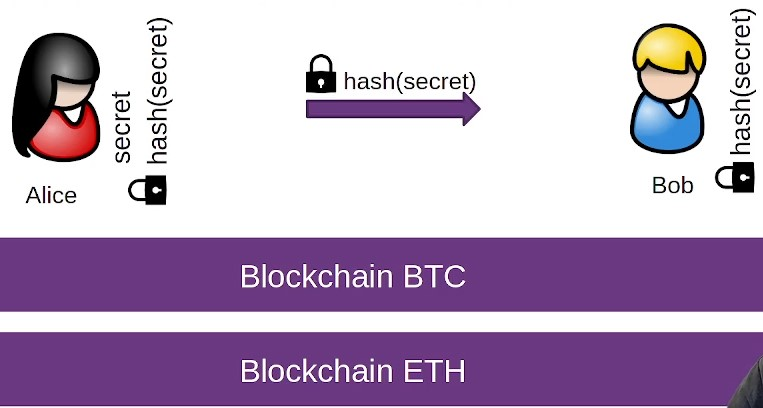
\includegraphics[width=\linewidth]{htlc-example-1.jpg}\\
Regular Case:\\
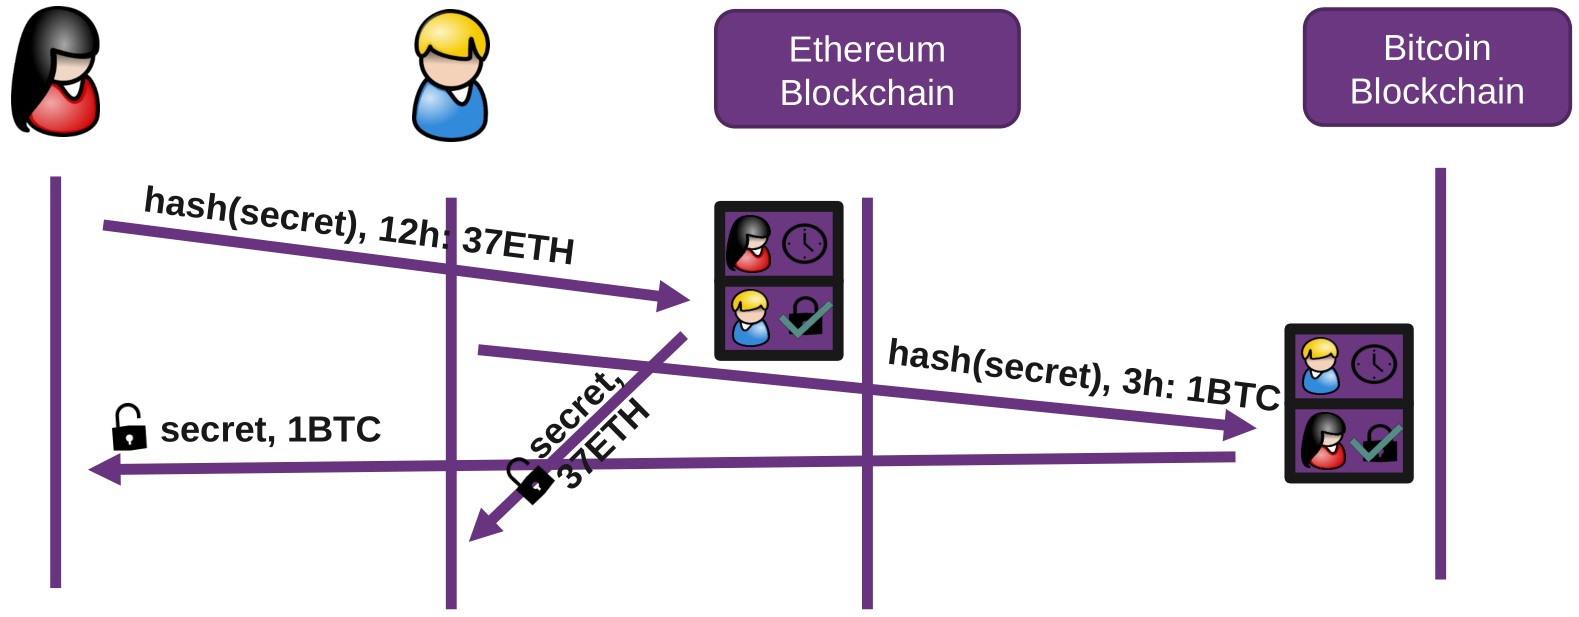
\includegraphics[width=\linewidth]{htlc-example-2.jpg}\\
Das Secret wird veröffentlicht. Wenn das Secret veröffentlich und eigesetzt wird, bekommt Bob die ETH.\\
Worst Case:\\
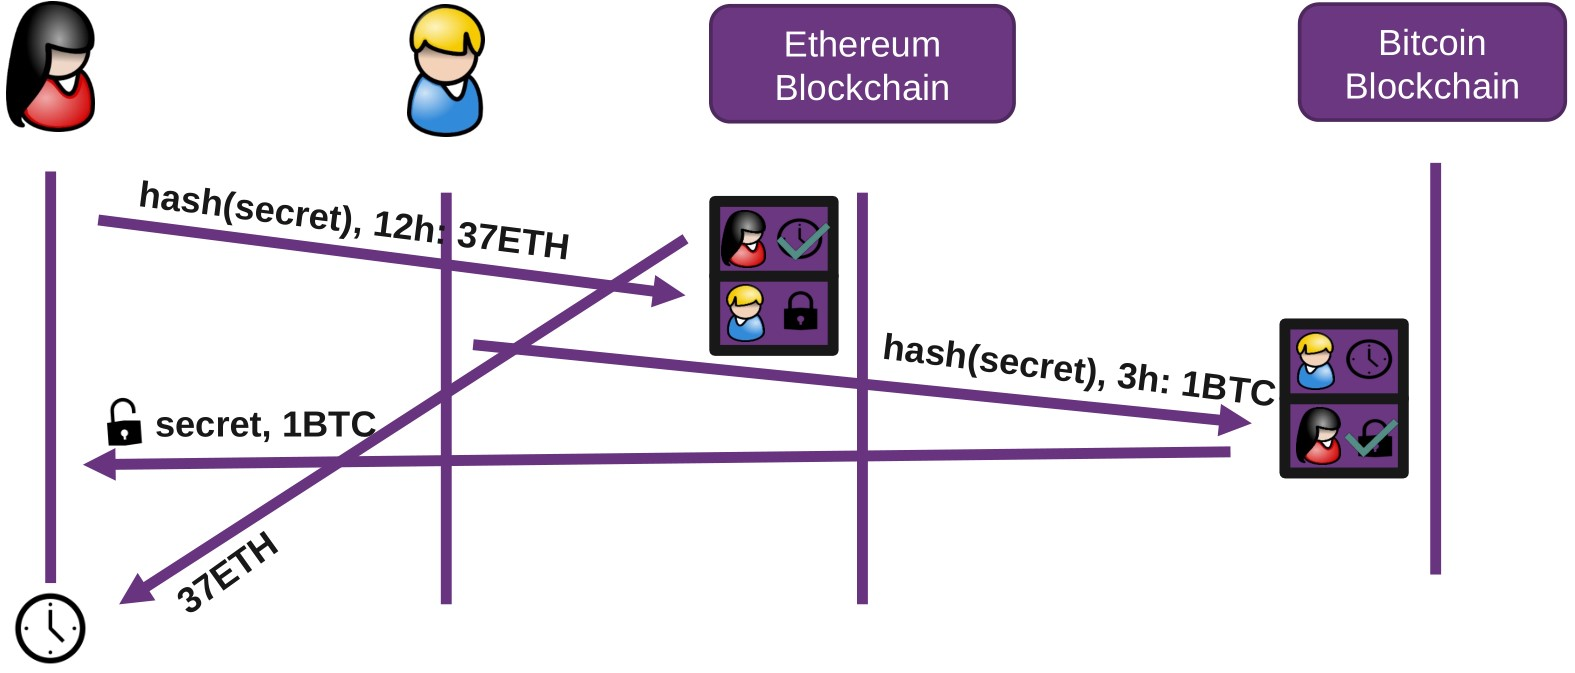
\includegraphics[width=\linewidth]{htlc-example-3.jpg}





\section{Layer 2 Payment Channels}
Blockchains grow linearly: Bitcoin Blockchain is 376.6 GB.
\subsection{Solutions}
\begin{itemize}
  \item First Layer Scalability Solutions
  \begin{itemize}
    \item Sharding (distribute storage)
    \item Improve protocol (SegWit, Taproot, Rollups)
  \end{itemize}
  \item Second Layer Scalability Solutions (off-chain)
  \begin{itemize}
    \item State Channels (payment channels): Lightning Network
    \item Sidechains / Blockchain Interoperability
  \end{itemize}
\end{itemize}

\subsection{2-of-2 Multisig}
Initial offchain TX.
Multiple transaction possible before everything is written to the blockchain.
Offchain transactions.
\subsubsection{Example}
1 BTC of Alice to Locked Multisig.
Alice can send 0.1BTC, then 0.2BTC, then the rest (or other constellation).
Bob can request some amount, then another amount (not exceeding Alice tho) as long as the multisig contract is open.\\
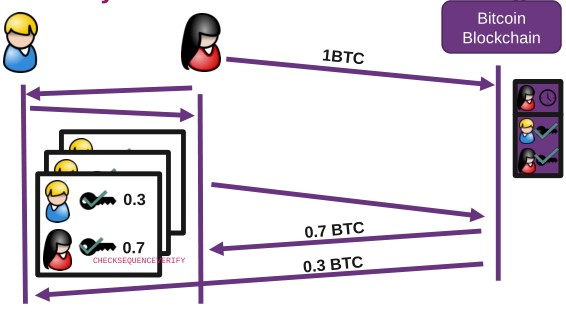
\includegraphics[width=\linewidth]{multisig.jpg}\\
After all transactions and when everyone's happy, both sign the contract and the total amount is given to the persons and the transaction is written to the blockchain.\\
For validation: CHECKSEQUENCEVERIFY. 

\subsection{Indirect Payment with HTLC}
Idea of Lightning Network.\\
1 BTC lockup, Alice - Bob, Bob - Charlie.\\
Alice wants to send 0.5 BTC to Charlie (no direct channel).\\
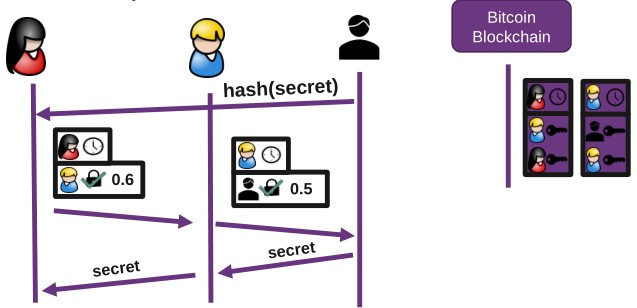
\includegraphics[width=\linewidth]{indirect-payment-htlc.jpg}
